\documentclass[../../lectures.tex]{subfiles}

\begin{document}

\chapter{Процессы}

\section{Общее}
\begin{itemize}
    \item Процесс --- экземпляр запущенной программы. Процессы должны уметь договариваться
          чтобы сосуществовать, но в то же время не знать друг о друге и владеть
          монополией на ресурс машины.
    \item С точки зрения ОС процесс --- это абстракция, позволяющая 
          абстрагироваться от внутренностей процеса.
    \item С точки зрения программиста процесс --- абстракция, 
          которая позволяет думать что мы монопольно владеем ресурсами машины.
    \item На момент выполнения процесс можно охарактеризовать полным состоянием его памяти
          и регистров. Чтобы приостановить процесс нам нужно просто сохранить его 'отпечаток', 
          а чтобы возобновить нужно загрузить его память и регистры.
    \item Батч-процессы (например, сборки или компиляции) не требуют 
          отзывчивости пока жрут ресурсы.
\end{itemize}

Могут быть сформулированы следующие тезисы:
\begin{itemize}
    \item Система не отличает между собой процессы
    \item Процессы в общем случае ничего не знают друг о друге
    \item Процесс - с одной стороны абстракция, которая позволяет не различать их 
          между собой, с другой - конкретная структура
    \item Память и регистры - однозначно определяют процесс
    \item Способ выбора процесса - алгоритм shedulerивания
    \item Переключение с процесса на процесс - смена контекста процесса
    \item Контекст процесса - указатель на виртуальную память и значения регистров
    \item Как отличать процессы между собой - \emph{pid}
\end{itemize}

\section{Модель памяти процесса}
\begin{figure}[H]
\begin{minipage}[c]{0.25\linewidth}
\centering
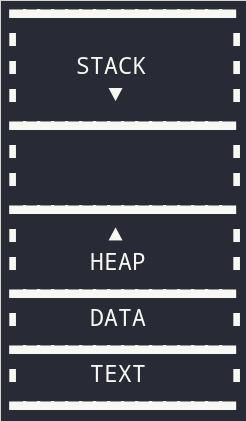
\includegraphics[width=\textwidth]{images/memory.png}
\caption{Memory in process}
\end{minipage}
\hspace{0.5cm}
\begin{minipage}[c]{0.7\linewidth}
\centering
\begin{itemize}
    \item \textbf{stack} --- выделяется неявно, \textbf{heap} --- должны выделять сами (malloc, new и тп),
    \item секции --- \textbf{data}, \textbf{text}
    \item \textbf{data} --- статические, глобальные переменные, \textbf{text}
    \item \textbf{stack} растет вниз, \textbf{heap} - вверх
    \item \textbf{frame} --- область памяти стека, хранящая данные об адресах возврата, информацию о локальных переменных
    \item Резидентная память та, которая действительно есть
\end{itemize}
\end{minipage}
\end{figure}

\section{PID и дерево процессов}
\begin{itemize}
    \item У каждого \emph{PID} есть parentPID (\emph{PPID})

    \item \shell{ps} --- позволяет посмотреть специфичные атрибуты процесса

    \item Процесс \emph{init(pid 0)} создается ядром и выступает родителем для большинства процессов, созданных в системе

    \item Можно построить дерево процессов (\shell{pstree})
\end{itemize}

Процесс делает \emph{fork()}. Возможны 2 случая:
\begin{enumerate}
    \item 
        Процесс не делает \emph{wait(childpid)}

        Зомби-процесс (\emph{zombie}) --- когда дочерний процесс завершается быстрее, чем вы сделаете wait
    \item 
        Процесс завершается, что происходит с дочерним процессом?

        Сирота (\emph{orphan}) --- процесс, у которого умер родитель. 
        Ему назначется родителем процесс с \emph{pid 1}, который время от времени делает \emph{wait()} и освобождается от детей
\end{enumerate}
\emph{PID} - переиспользуемая вещь (таблица процессов)

\section{Системные вызовы для работы с процессами}
\begin{itemize}
    \item \emph{fork()} --- для того чтобы создать новый процесс
    \code{fork-example.c}{C}
    \emph{fork}-бомба --- каждый дочерний процесс делает \emph{fork()} и так далее
    \item \emph{wait(pid)} --- ждем процесс
    \item \emph{exit()} --- завершаемся
    \item \emph{execve()} --- запустить программу
    \code{execve-example.c}{C}
    \item \emph{kill()} --- послать сигнал процессу
    \item \emph{SIGKILL} --- сигнал для принудительного завершения другого процесса 

          \shell{kill -SIGKILL pid} 
\end{itemize}

\section{Calling convention}
\shell{man syscall} - как вызываются \emph{syscall}

\code{syscall.h}{C}
\code{syscall.s}{asm}
\code{syscall-example.c}{C}

Что здесь просходит?
\begin{enumerate}
    \item Вызываем write()
    \item Просим ядро записать 555 байт начинающихся по адресу 0 в файловый дескриптор №1 
          (\emph{stdout} --- №1, \emph{stdin} --- №2, \emph{stderr} --- №3)
    \item Ничего не происходит, так как:

          \emph{write(1, NULL, 555)} возвращает -1 (\emph{EFAULT} - Bad address)
\end{enumerate}

Как со всем этим работать?
\begin{itemize}
    \item \shell{strace} --- трассировка процесса (подсматриваем за процессом, 
          последовательность \emph{syscall} с аргументами и кодами возврата)

    Если \emph{syscall} ничего не возвращает, то в выводе пишется ? вместо возвращаемого значения

    \item \shell{man errno} --- ошибки

    Если делаем \emph{fork()} --- проверяем код возврата (хорошая практика)

    \emph{char* strerror(int errnum)} - возвращает строковое описание кода ошибки

    Почему \emph{char*}, а не \emph{const char*}? Потому что всем было лень.

    \emph{thread\_local} --- решение проблемы: переменная с ошибкой - общая для каждого потока

    \item До \emph{main()} и прочего (конструкторы) происходит куча всего 
          (\emph{munmap, mprotect, mmap, access}) - размещение процесса в памяти и т.д.

    \item Программа не всегда завершается по языковым гарантиям (деструкторы)

    \item \shell{ptrace} --- позволяет одному процессу следить за другим (используется, например, в \emph{GDB})

    \item \emph{ERRNO} --- переменная с номером последней ошибки, strerror

    \item \emph{finalizers}, библиотечный вызов \emph{exit}
\end{itemize}

\section{API and ABI}
\begin{itemize}
    \item \textbf{API} (Application Program Interface)\\
          Интерфейс коммуникации на уровне исходного кода
          (include, functions, etc)
    \item \textbf{ABI} (Application Binary Interface)\\
          Интерфейс коммуникации на бинарном уровне
          (как параметры передаются функциям, кто очищает
          параметры функции и т.д.)
\end{itemize}

\section{Процесс и ОС}
\subsection{Scheduler}
\begin{itemize}
    \item Заводит таймер для процесса(квант времени), после его истечения 
    или когда процесс сам закончился выбирает другой процесс.

    \item Производительность - разбиение на несколько процессов

    \item Дизайн приложения
\end{itemize}
\subsection{Interruption}
\centerimage{process-interruption.png}{Interruption of process}{0.8}

\subsection{Состояния процесса}
\begin{figure}[H]
\begin{minipage}[c]{0.6\linewidth}
\centering
\includegraphics[width=\textwidth]{images/state-diagram.png}
\caption{Диаграмма жизни процесса}
\end{minipage}
\begin{minipage}[c]{0.4\linewidth}
\centering
Процесс может быть в одном из следующих состояний
\begin{itemize}
    \item \textbf{runnable}
    \item \textbf{running}
    \item sleeping: \textbf{interruptible}
    \item sleeping: \textbf{uninterruptible}
    \item \textbf{zombie}
    \item \todo{maybe not all}
\end{itemize}
\end{minipage}
\end{figure}

\subsection{Контекст процесса}
\begin{itemize}
    \item Память
    \item Вычислительный контекст --- потоки
    \item Файловые дескрипторы (открытые файлы и сокеты)
    \item \textbf{IPC}
    \item \textbf{Credentials} (\shell{man 7 credentials})
\end{itemize}
\todo{Подробнее}

\subsection{Переключение контекста}
Шедулер ОС раскидывает процессы и создает иллюзию одновременного выполнения
\centerimage{context-switch.png}{Иллюзия многозадачности}{0.5}

\section{Системные процессы}
\todo{What is this?}
\begin{itemize}
    \item kthreadd
    \item kswapd
    \item ksoftirqd
\end{itemize}

\newpage
\section{Литература}
\begin{itemize}
    \item Windows Internals by Mark Russinovich
    \item Операционная система UNIX. Андрей Робачевский
    \item Unix и Linux. Руководство системного администратора. Эви Немет.
\end{itemize}

\section{Домашнее задание №1} 
Необходимо создать игрушечный интерпретатор.

Цель --- получить представление о том, как работают командные интерпретаторы.
\begin{itemize}
    \item Программа должна в бесконечном цикле считывать с \emph{stdin} полный путь к
          исполняемому файлу, который необходимо запустить и аргументы запуска.
          Дождавшись завершения процесса необходимо вывести на stdout код его завершения.

    \item Необходимо использовать прямые системные вызовы для порождения новых процессов,
          запуска новых исполняемых файлов и получения статуса завершения системного
          вызова.

    \item Все возвращаемые значения системных вызовов должны быть проверены и в случае
          обнаружения ошибок необходимо выводить текстовое описание ошибки.

    \item На входе могут быть некорректные данные.

    \item Дополнительные баллы - поддержка переменных окружения.

    \item Язык имплементации - C или C++.
\end{itemize}
\end{document}
